\chapter{Substructure Discovery in Tandem Mass Spectometry Data}
\label{c:background}

\note{Around 20 pages}

\section{Introduction}

Untargeted metabolomics studies have the potential to answer important questions in many areas of the life sciences. Unfortunately, this potential is not fully realized due to the lack of computational tools that are able to extract the key biochemically relevant information from a particular assay, or set of assays (from e.g. a clinical trial). \textbf{As discussed in Chapter XX, identificatication can be performed through ID of the fragmentation spectra. MS1 .. is what? Fragmentation spectra, produced through the tandem-MS process, is also referred to as MS2 peaks.| } Most computational tools being being produced focus on identifying/annotating molecules from fragmentation spectra, with identified molecules being kept for subsequent analysis. Although annotations from fragment spectra have clear utility, in even the most widely studied organisms, the majority of molecules cannot be identified in this way. Spectra that cannot be identified are therefore of no use in this type of analysis, despite the fact that they must include information relevant to the biochemical processes taking place within the organism. 

Despite the focus on it, metabolite identification is rarely the end-goal in an untargeted metabolomics analysis. Rather, it is a route to understanding the biochemistry (and changes in biochemistry) within the system under study. For example, identified molecules are mapped to pathways whose relative activity can be estimated from fold changes of the individual molecules. Consequently, poor identification coverage results in poor biochemical insight. Fragmentation spectra contain recurring patterns of fragments and losses due to the presence of common biological substructures (e.g. a hexose unit, or a CO loss). Here, each observed spectrum is assumed to be comprised of one or more of these substructures. The representation of small molecules as combinations of building blocks has previously been used for the annotation of a small number of molecules in direct infusion-MS with fragmentation [27] and for metabolite classification in GC-MS [28, 29]. CSI:FingerID ranks candidate molecules based on the presence and absence of various predefined structural features, including substructures [5]. These studies reveal the potential of substructure-based approaches in MS but require structurally known training data, which is costly to produce and often platform-specific. 

In this chapter, we propose an alternative analysis workflow that reduces the large number of fragmentation spectra to concurring patterns of mass fragments or neutral losses to which precursor ions are associated. This is accomplished through the application of the Latent Dirichlet Allocation (LDA) model to spectral fragmentation data. The proposed workflow, called 'MS2LDA', uses all fragmentation data from a particular assay to extract biochemically-relevant features in an unsupervised manner (i.e. without large volumes of training data). Our approach extracts biochemically-relevant molecular substructures (‘Mass2Motifs’) from a collection of fragmentation spectra as sets of co-occurring fragments and neutral losses. This analysis allows us to immediately explore the biochemistry present in the sample via the relative abundance of a small number of different molecular substructures that, based on our analysis, are often straightforward to annotate. The presence of shared substructures allows us to group molecules in a meaningful way even if they do not share a large degree of overall spectral similarity. If many molecules in such a group share a pattern of differential expression, we can hypothesise the cause of the change in abundance without having to identify all of the molecules and map them to a metabolic pathway. Presence of substructures can also be used to provide putative annotations (or functional classifications) for molecules that are otherwise unidentifiable. 

Our results demonstrate that the proposed approach can extract structural features in the form of sets of mass fragments and neutral losses in an unsupervised manner without any a-priori knowledge. This is not something that can be done with any of the current metabolomics analysis tools. We conclude that the resulting workflow allows a researcher to focus on relevant fragmentation patterns in data-dependent mass spectrometry fragmentation files and use them as aid in metabolite annotation and classification. The results from structural annotations of multiple sample performed independently also suggests a useful extension to the standard LDA model, where the presence of Mass2Motifs across many samples can be jointly inferred, allowing changes to their expression levels to be compared easily.

\section{A Workflow for Substructure Discoveries and Annotations}

The key insight of the MS2LDA workflow lies in the parallels between text and MS fragmentation data (Figure~\ref{fig:text2frags}) that motivates our approach. As a text analysis pipeline relying on LDA decomposes documents into topics based on frequently co-occurring words, so MS2LDA decomposes fragmentation spectra into their constituent building blocks of frequently co-occurring fragments and neutral losses (referred to as ‘Mass2Motifs’). Crucially, MS2LDA achieves this with a purely data-driven approach. By using all of the fragmentation spectra generated by data-dependent mass fragmentation analysis (DDA), it learns the conserved substructures (the Mass2Motifs) and the decomposition of the fragmentation spectra (into Mass2Motifs).  

\begin{figure}[!htbp]
\centering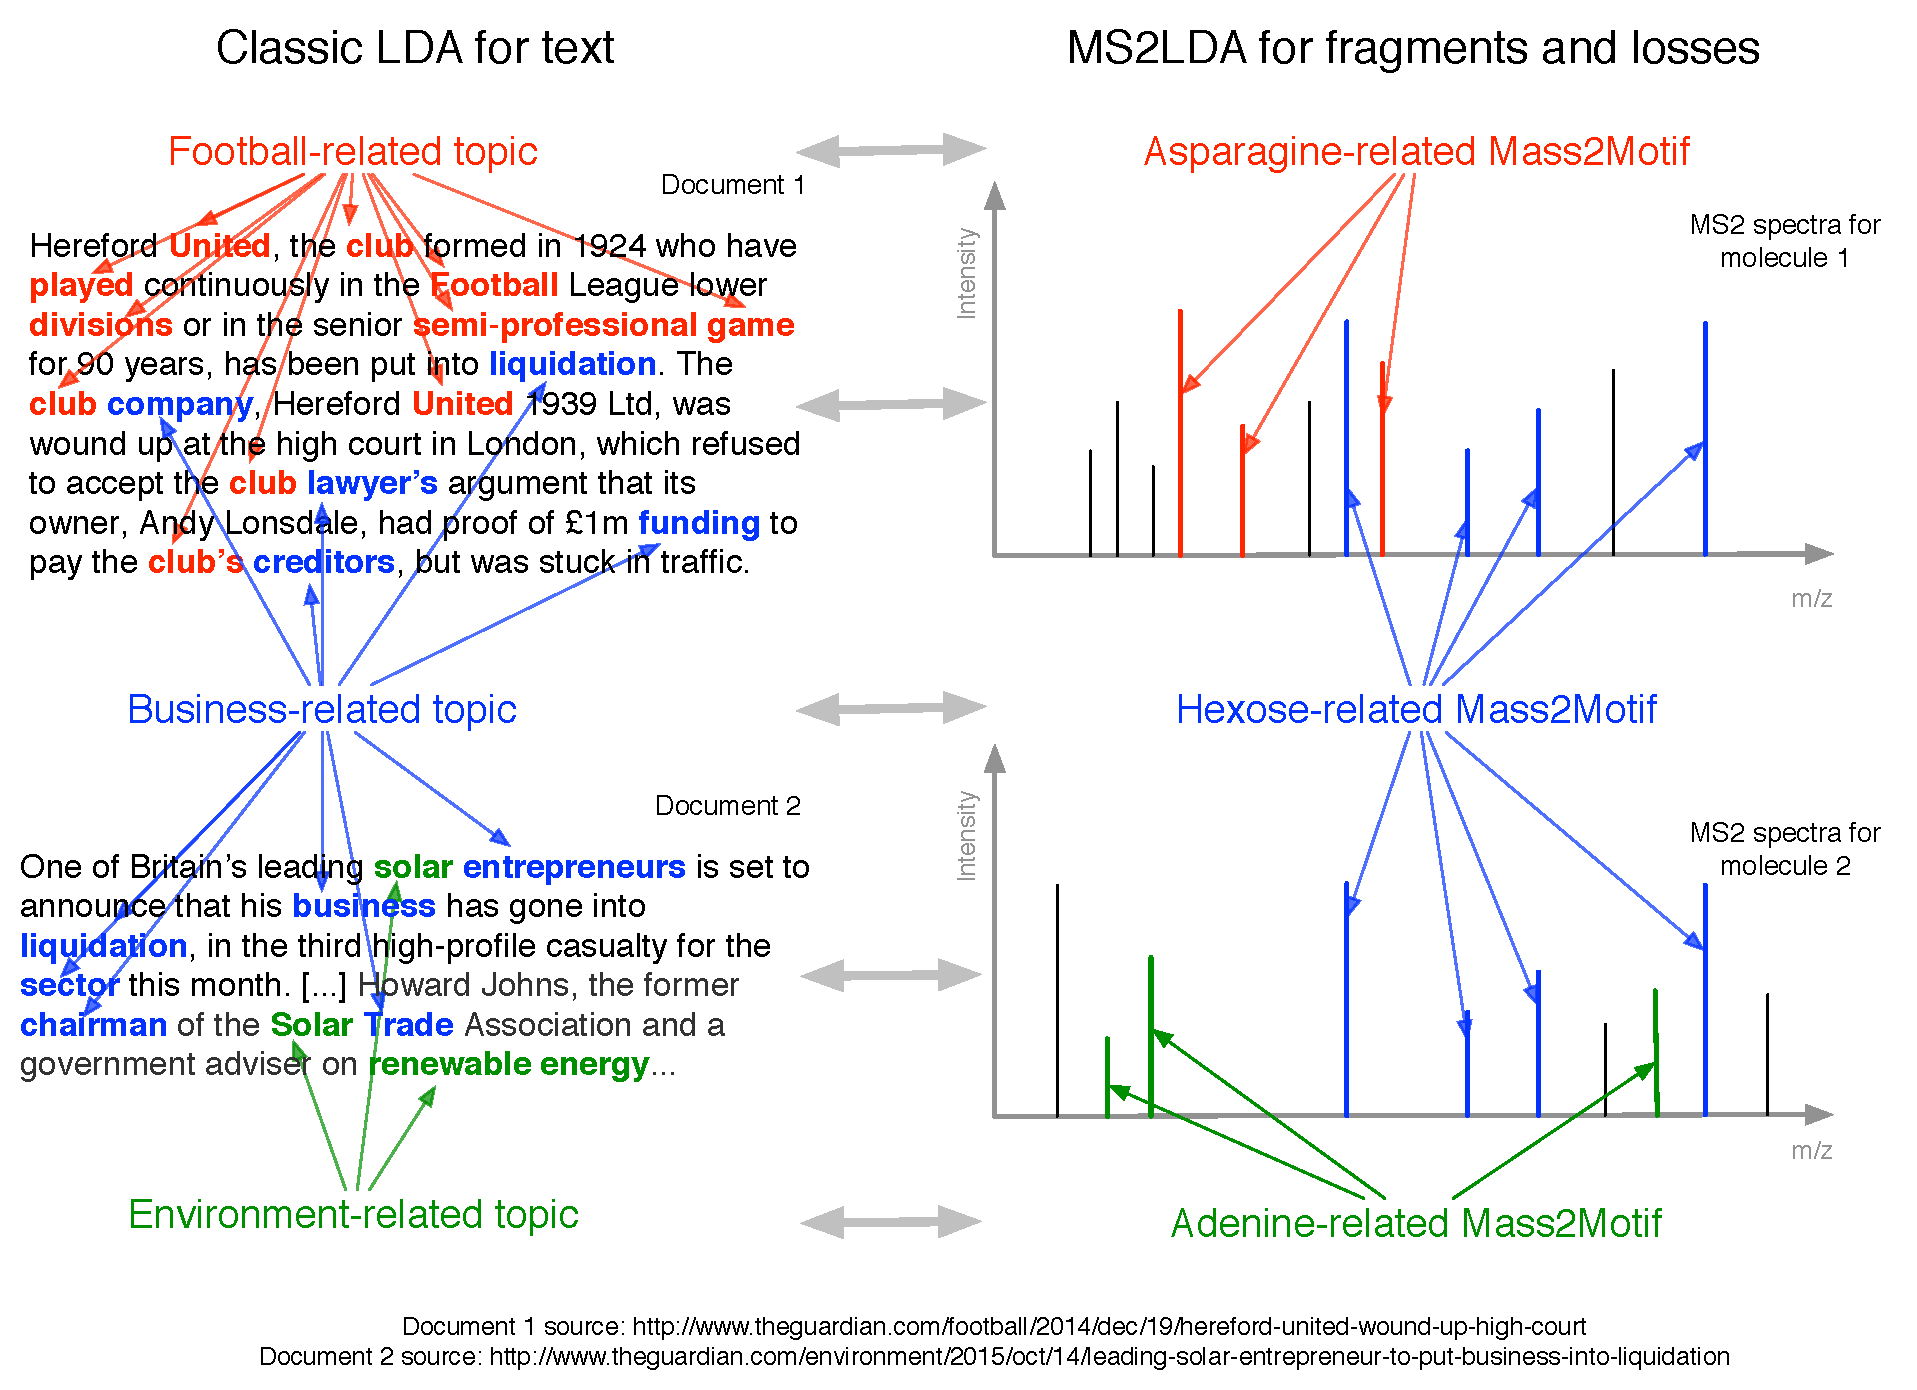
\includegraphics[width=0.7\linewidth]{07-lda/figures/text2frags.pdf}
\centering\caption{Figure 1: Analogy between LDA for text-mining and MS2LDA. In this example, we can see that traditional LDA has extracted topics that can be interpreted as ‘football related’, ‘business-related’ and ‘environment related’. Each document is a combination of different topics. In a similar manner, MS2LDA extracts different sets of concurring mass fragments or losses (Mass2Motifs) from the fragmentation spectra of precursor ions that can be interpreted as ‘Asparagine-related’, ‘Hexose-related’ and ‘Adenine-related’. Each fragmentation spectra is made up of one or more Mass2Motifs.\label{fig:text2frags}}
\end{figure}

The MS2LDA workflow consists of two stages: i) the data conversion stage, which prepares the acquired fragmentation data into suitable input format for the workflow, followed by ii) the Mass2Motif discovery stage, which performs topic modelling via LDA to discover mass fragmental patterns, assigns potential candidate elemental formulae to MS1 and MS2 peaks, and visualises the Mass2Motifs in an interactive environment. The complete MS2LDA workflow is schematically illustrated in Figure~\ref{fig:m2lda-workflow} and described in more details in the following.

\begin{figure}[!htbp]
\centering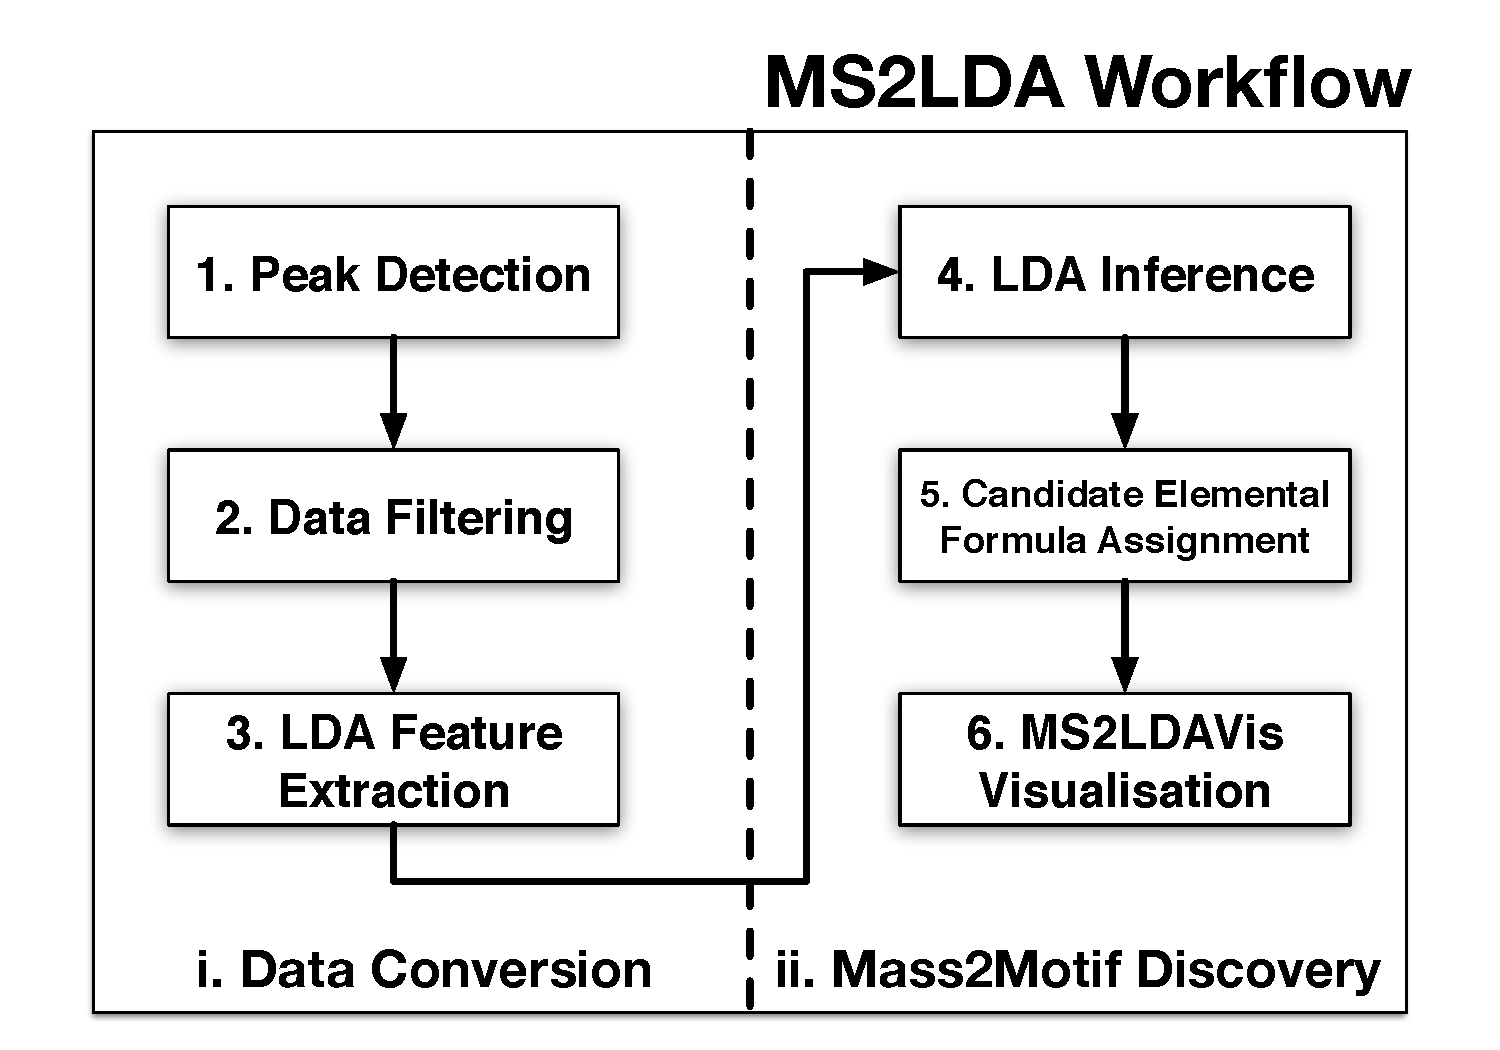
\includegraphics[width=0.7\linewidth]{07-lda/figures/ms2lda.pdf}
\centering\caption{Schematic overview of the MS2LDA workflow..\label{fig:m2lda-workflow}}
\end{figure}

\subsection{Data Conversion}

\subsubsection{Peak Detection \& Data Filtering}

Data conversion is an essential part of the MS2LDA workflow, since the acquired fragmentation data cannot readily be used for the purpose of mass fragmental pattern searching. Our workflow accepts as input the combination of a single full-scan file for the MS1 peaks and a separate fragmentation file for the MS2 peaks (alternative strategies for peak detection and MS1-MS2 correspondence establishment that accept different combinations of input files, such as using just a single fragmentation file for both the MS1 and MS2 peaks, are also provided in our workflow). The data conversion process starts with the detection of MS1 peak in the input .mzXML file obtained from full-scan mode spectra using the CentWave algorithm from the XCMS library [2]mzML file obtained in MS/MS mode are then established using a script based on the RMassBank package [3] through greedy search for the most intense unique MS2 spectrum (more intense fragmentation spectra are generally information-richer) that can be linked to an MS1 LC-MS peak within a specified retention time (RT) window. A filtering step based on RT and intensity is applied to remove noisy peaks, as well as the washing part, equilibration part, and the start of the chromatogram prior to the injection peak. Finally, any MS1 peak not having paired MS2 peaks is discarded. This process leaves unique MS1-MS2 pairs, thereby omitting the lower intense fragmentation spectra of MS1 peaks that were fragmented multiple times. This greatly helps in the LDA modelling, as multiple spectra of the same MS1 peak could  be considered as conserved mass fragmental motif in the data set.

\subsubsection{LDA Feature Extraction}

The next step in the data conversion stage is the transformation of the spectral data into a format that is suitable for concurring pattern discovery, which is a matrix consisting of the MS1 peaks (columns) and their correspondent MS2 fragments (rows), see Figure S-1, or losses. Drawing an analogy from text mining, each MS1 peak can now be seen as a ‘document’ while the linked MS2 spectrum associated to each MS1 peak produce the ‘words’ in a document. Note that LDA does not take into account the word order, but merely the ‘word count’, i.e., the number of times a word occurs in a document. For each MS1 peak, two types of features can be extracted from the MS2 fragmentation spectrum:

•	Fragment features, which are the discretized mass values of the MS2 peaks. A greedy binning process is used to group MS2 peaks within a certain user-defined m/z window from the next unprocessed MS2 peak. This way, MS2 peaks with close-enough m/z values but observed in different precursor MS1 peaks are linked and placed into the same discrete bin – each bin corresponds to a fragment feature. The input for inference in textual LDA is the count of occurrences of words in each document; in MS2LDA, the intensity values of MS2 peaks can be considered to be proxies for word counts. These intensity values are normalized by dividing to the largest intensity value in the fragmentation spectrum and discretized on a scale of 0 to 100 (integers). 

•	Loss features, which is the discretized mass values of the neutral losses. Neutral losses are the mass differences between a precursor MS1 peak and each of its MS2 peaks in the spectrum. To produce the loss features, we find the m/z difference between each fragment peak to its precursor ion. Similar to fragment features, the normalized intensity values of the neutral losses, represented by the intensities of their resulting mass fragments, are used as proxies for the loss counts.

\subsection{Mass2Motif Discovery}

\subsubsection{LDA Inference}

Given the data-frames produced from the data conversion, our goal now is to infer the concurring patterns of features shared by the fragmentation spectra. Following the Latent Dirichlet Allocation (LDA) model, a fragmentation spectrum can be seen as a mixture over potentially substructure patterns (which we called Mass2Motifs), each of which is itself a distribution over fragment/loss word features. A fragmentation spectrum, linked to a particular MS1 peak, can therefore be generated in this model by firstly sampling for the Mass2Motifs that the spectrum is comprised of and subsequently sampling the specific fragment/loss features from the selected Mass2Motifs. Following Section~\ref{background-lda}, a Python implementation of a collapsed Gibbs sampling scheme is used for inference in our MS2LDA workflow. In this particular case of LDA inference, the input to Gibbs sampling is the observed counts of fragment/loss words co-occurrences in fragmentation spectra (documents) and as output, we infer the latent Mass2Motif-to-words distributions and fragmentation spectra-to-Mass2Motif distributions present in the data. In our Gibbs sampling implementation, only the last sample (after monitoring for convergence) was used for the purpose of analysis. Due to the stochastic nature of the Gibbs sampling procedure, we might get slightly different results each time, which may be undesirable. To overcome this, we set a constant random seed for the sampler, allowing us to get the same inference results each time, provided the same parameters are used with the same input files.

\subsubsection{Candidate Elemental Formula Assignment}

The MS2LDA workflow provides two optional methods to assign candidate elemental formulae to the mass fragments, neutral losses, and precursor ions. The first is achieved by integrating SIRIUS (Sum formula Identification by Ranking Isotope patterns Using mass Spectrometry, [6]) into our workflow. SIRIUS assigns elemental formula by posing it as an integer decomposition problem and solving it through a dynamic programming approach ('Round Robin') [7]. SIRIUS is freely-available and, as it is written in Java, can in theory be run platform-independently on any Windows, Unix and Mac environment (in practice, library dependencies have to be satisfied before SIRIUS can be run on the target computer). Integration of SIRIUS into our workflow is achieved by wrapping calls to the Java package of SIRIUS through a separate sub-process, passing it a temporary MGF file that corresponds to each fragmentation spectrum. SIRIUS assigns elemental formulae to each combination of MS1 and MS2 peaks independently, which may lead to mass fragments of similar m/z value being assigned an elemental formula in some spectra, but not in all.

As an alternative strategy for annotation, our workflow also provides a pure Python implementation of an elemental formula assigner (called 'EF-Assigner') based on the Round Robin algorithm that also lies at the heart of SIRIUS. Once the initial assignment of potential candidate formulae to mass fragments, neutral losses and also precursor ion masses has been performed, the list of candidate formulae is further filtered using our implementation of the 7-golden rules, a set of heuristic rules introduced by Kind and Fiehn [8]. This filtering step is used to remove chemically-unlikely elemental formula compositions from the candidate list. Advantages of the EF-Assigner module are its easy compatibility (it is also written in Python) and it assigns elemental formulae to the binned fragments and losses in the matrix instead of to individual spectra. However, unlike SIRIUS that uses the complete information of the precursor ion and fragments peaks in a spectrum for annotation, EF-Assigner assigns the elemental formulae for the MS1 peaks, mass fragments and neutral losses independently. 

\subsubsection{MS2LDAVis Visualisation}

Inference results from LDA can be challenging to interpret due to the (still) high dimensionality of the data. Analysis of Mass2Motifs to examine if they correspond to actual structural features or biochemical substructures is an iterative and exploratory process. In our workflow, this is made possible through the MS2LDAVis module -- an interactive web-based visualization that can be used to explore and validate Mass2Motifs in MS2 data. MS2LDAVis is extended from the Python port of the topic modelling visualization interface LDAVis [9], which is built upon the combination of the Javascript/D3 library and Python. 

Similar to the original LDAVis, the left panel of our MS2LDAVis module shows a global view of the model, whilst the right panel zooms into a specific Mass2Motif (see Figure S-2). However, unlike LDAVis where topics are displayed on the left panel through multidimensional scaling that projects topics to two dimensions, the two axes in our MS2LDAVis panel are the log-degree and the h-index of Mass2Motifs. We defined the degree of a Mass2Motif as the number of fragmentation spectra explained by the Mass2Motif at the user-defined thresholding level  on the fragmentation-spectra-to-Mass2Motif distributions (the θ parameters). The -index of a Mass2Motif is defined in a similar manner to the conventional h-index for scientific publications of a researcher. A Mass2Motif has an index of  if it has  fragment/loss features obtained after setting a user-defined threshold  on the Mass2Motif-to-word distributions (the φ parameters), each of which occur in the set of thresholded documents at least  times. Intuitively, Mass2Motif with high degrees but low -index could potentially correspond to simple structural features or substructures that occur in many MS2 fragmentation spectra, while Mass2Motif with high -index but lower degrees could potentially correspond to more unique and complex substructures shared by fewer MS2 spectra.

Figure S-2. Screenshot of MS2LDAVis. See text for explanations of the different panels.

Similar to LDAVis, the left and right panels of our visualization are linked such that selecting a Mass2Motif on the left changes the information displayed on the right panel. We further enhanced MS2LDAVis by plotting the fragmentation spectra of each MS1 peak (documents) above the user-defined threshold  in the selected Mass2Motif. The fragment and loss words in the fragmentation spectra that are explained by the currently selected Mass2Motif, i.e., above the user-defined threshold , are highlighted in bold and user can easily flip through different fragmentation spectra explained by the topic by clicking the ‘Previous MS1’ and ‘Next MS1’ buttons. The bottom of the right panel displays two feature frequency histograms; the Mass2Motif Feature Frequencies histogram displays the counts of each Mass2Motif associated fragment or loss (above the user-defined threshold  on the Mass2Motif-to-word distributions [the φ parameters]) within the fragmentation spectra explained by the Mass2Motif. Similarly, the Global Feature Frequencies histogram display the overall frequency of the fragments or losses within the complete data set that can be explained by the currently selected Mass2Motif. This provides an estimate of how unique the fragment/loss features are in the whole data set.

Finally, to complement our main view, we also allow the possibility of exploring the inferred substructure data in a pop-up network graph (Fig. S-3), where Mass2Motifs and MS1 peaks form the nodes in the graph and edges are drawn between them if a document is explained by a topic with conditional probability above the user-defined threshold . The graph view can be accessed by clicking on the ‘Show Graph’ button in the main visualization window. To minimize clutter in the network graph, user can also define a threshold on the degree of the Mass2Motifs, i.e., all Mass2Motifs with a degree of 10 or lower can easily be removed from the graph. Nodes in the graph can also be annotated and coloured according to user-defined specifications before the visualisation interface is called (see Figure S-3). The two complementary views are linked such that clicking a topic node on the network graph will select the corresponding topic on the main view and vice versa. The network graph is particularly useful in exploring the relationships between Mass2Motifs and investigating which MS1 peaks have fragmentation spectra that can be explained by multiple Mass2Motifs.

Figure S-3. MS2LDAVis network graph of beer3 extract positive ionization mode file where a number of Mass2Motifs were selectively colored before loading the network visualization. Mass2Motifs circles are proportional to their degree (number of connections), whereas small blue squares represent fragmented MS1 peaks.


\section{Evaluation Study}

\subsection{Evaluation Datasets}

The MS2LDA workflow was independently applied to four complex biomolecular mixtures in the form of beer extracts. A standard peak-picking metabolomics data processing workflow, based on XCMS and MzMatch [31, 39], was used to match MS1 with MS2 spectra. We obtained, on average (across the four datasets), 1409 and 1125 fragmented MS1 peaks in positive and negative ionization mode respectively (see Supporting Information section 5.1 for more details). These fragmentation pattern were analysed with Latent Dirichlet Allocation (LDA) and the results, i.e. ‘Mass2Motifs’, were explored using the MS2LDAvis environment.

We used beer samples as representative of complex mixtures of diverse biochemically relevant compound classes like amino acids, nucleotides, and sugars. Beer extracts were acquired from three different commercially available beers and one home-brewed beer: Beer1 is sampled from a home-brewed bottle of German Wheat Beer of which the Beer sheet is available (see section 1 in the Supporting Information); Beer2 is sampled from a bottle of ‘Jaw Glyde Ale’ (a Golden/Blond Ale) brewed by JAW Brew (http://www.jawbrew.co.uk); Beer3 is sampled from a bottle of ‘Seven Giraffes Extraordinary Ale’ (an IPA style of beer) brewed by William Bros. Brewery Company (http://www.williamsbrosbrew.com/beerboard/bottles/seven-giraffes); Beer4 is sampled from a bottle of ‘Black Sheep Ale’ (a Golden Bitter Ale)  (https://www.blacksheepbrewery.com/beers/15/black-sheep-ale).

Approximately 10 ml of beer was sampled from each bottle directly after opening and stored at -20 ˚C before extractions. After thawing, i) 200 µL of beer was mixed with 600 µL of methanol/chloroform, ii) then sonicated for 5 minutes at room temperature; iii) and finally centrifuged for 5 minutes (12,000 g) at room temperature. As well as the four individual extracts, a pooled aliquot of the four beer extracts was prepared. The resulting supernatants were stored at -80 ˚C until analysis.

A Thermo Scientific Ultimate 3000 RSLCnano liquid chromatography system (Thermo Scientific, CA, USA) was used. That system was coupled to a Thermo Scientific Q-Exactive Orbitrap mass spectrometer equipped with a HESI II interface (Thermo Scientific, Hemel Hempstead, UK). Thermo Xcalibur Tune software (version 2.5) was used for instrument control and data acquisition.

Positive Negative Ionization Combined Fragmentation Mode:
A duty cycle consisted of a full scan in positive ionization mode, followed by a TopN data dependent MS/MS (MS2) fragmentation event taking the 10 most abundant ion species not on the dynamic exclusion list, followed by the same two scan events in negative ionization mode. More details can be found in section 2.1 of the Supporting Information. Most importantly, MS/MS fragmentation spectra were acquired using stepped higher collision dissociation (HCD) combining 25.2, 60.0, and 94.8 normalized collision energies (NCEs) in one MS2 scan.

The workflow was adapted from Creek et al., 2011, where samples were measured in randomized order [30]. Details can be found in section 3 of the Supporting Information.

The MS2LDAVis module can be used to analyse and explore the discovered Mass2Motifs in the resulting project files (for details, see section 4.4 of the Supporting Information). To aid in visualization and exploration, the distributions over the features that make up the Mass2motifs and the distributions over Mass2motifs for each fragmentation spectrum can be thresholded. The default threshold values were manually selected for visualization but can be varied. In our analysis, Mass2Motifs with degrees ≥10 (i.e. that were present in ten or more spectra after thresholding) were manually inspected and annotated at different levels of confidence (see Table captions of Supporting Tables S-1 and S-2). Annotations of Mass2Motifs were established through expert knowledge and by spectral matching of the MS2 spectra containing the associated fragments and/or neutral losses to the reference spectra in MzCloud (www.mzcloud.org). Key fragment or loss features from the annotated Mass2Motifs in one sample were then searched against the list of Mass2Motifs in other samples and their correspondences established if those key fragment/loss features were present in both.

\subsection{Model Comparison}

The number of motifs and model fit are estimated via a 4-folds cross-validation approach. For each test fold being held out in the fragmentation spectra data set, an estimate of the model evidence is computed after training the model on the remaining training folds in the data set. A common comparison of LDA is against the multinomial mixture model (clustering). A crucial difference between LDA and standard mixture-model clustering lies in the modelling assumption that a document is a mixture of one or more topics (LDA) as opposed to each document having exactly one topic (clustering). We compare the model fit of LDA against clustering by evaluating the log evidence and perplexity on a held-out beer data file (beer3 positive ionization mode). The perplexity measures how well a probability distribution or probability model predicts a sample and defined as:

$perplexity(W)=exp(...)$

Where  is the perplexity on the whole held-out test collection,  is the marginal probability of a testing document d (integrating over all the parameters of the model), approximated via an importance sampling method as described by Wallach et al. [5] and  is the number of words in each testing document . We follow Griffiths and Steyvers [4] and set the value of the hyperparameters α =K/50 and β =0.1 for LDA during the cross-validation experiment. For mixture model clustering, a non-informative Dirichlet prior (with constant parameter α =K/50, where K is now the number of clusters) is set on the proportions of the mixture components and another Dirichlet prior (with constant hyper-parameter β =0.1) is set on cluster-specific word distributions. The Gibbs sampler for LDA and multinomial mixture model is run for 1000 samples, discarding the first 500 for burn-in. The lower perplexity (shown in Figure 7 of the main document) demonstrates that LDA provides a better model fit on the held-out data compared to multinomial mixture model.

\section{Results \& Discussion}

\subsection{Model Comparison Results}

\subsection{Biological Findings}

300 Mass2Motifs were extracted for each data file. MS2LDA indeed found recurring mass fragmentation patterns that were checked for biochemical relevance. 30-40 Mass2Motifs in each of the positive ionization mode files were structurally annotated (see Supporting Tables S-1 and S-2). Examples of the biochemically relevant and diverse substructures we found include histidine, phenylalanine, adenine, and a hexose-unit, as well as structural features such as water or carboxyl group loss. Although MS2LDA reduces the complexity of large fragmentation datasets, the output of is still complex (>1000 precursor ions and ~300 Mass2Motifs). To overcome this, we have developed an interactive visualisation tool that enables rapid exploration of the MS2LDA output. 

Figure 7 – A subset of the network produced by MS2LDA and displayed by the visualisation tool. The network is a bipartite graph with two sets of nodes, corresponding to the Mass2Motifs (circles) and the parent ions (squares). An edge indicates that a Mass2Motif is found in the spectrum of the parent ion. Parent ions and Mass2Motifs can be sized and coloured according to different characteristics of the data. In this example the parent ions have been coloured according to their fold change between two MS1 datasets of beer extracts (red if >2.72, green if <0.37, black otherwise) and the Mass2Motifs have been sized according to the differential expression score from PLAGE analysis.

The visualisation tool consists of several panels, each of which provides a different view on the MS2LDA output. The first is a network (a subset of which with various Mass2Motifs highlighted is shown in Figure 7). Selection of a Mass2Motif in the network allows the user to view all spectra associated with that Mass2Motif in a separate panel with relevant fragments and neutral losses highlighted (in the style of e.g. Figures 3 and 4). In the final panel, the MS2LDAvis environment shows frequency histograms that can be used to determine how consistently present the conserved fragments or losses are within the Mass2Motif. Examples for histidine related Mass2Motifs found in two of the beer extracts can be seen in Figure 8.

Figure 8 – Similar sets of fragment and loss features can be seen in the MS2LDAVis ‘Mass2Motif Feature Frequency’ histograms for histidine-related Mass2Motifs in positive mode of beer1 (top) and beer3 (bottom). The left-hand panels show the number of times each feature appears in spectra associated with this Mass2Motif while the right-hand panel shows the proportion (red) of the total abundance (blue) of this feature within the dataset explained by this Mass2Morif. For example, this Mass2Motif accounts for the vast majority of the total abundance observed for the fragment with mass 110.0718. Conversely, although the fragment with mass 95.0608 appears often in the spectra associated with this Mass2Motif, it appears widely elsewhere too. Because the analyses of the four beers were done separately, fragment masses do not exactly match across samples. 

The ‘Mass2Motif Feature Frequencies’ histograms (Figure 8-A, 8-C) display how often particular fragments or losses appear in spectra including this Mass2Motif, indicating their consistency. For example, from Figure 8-A and 8-C we can see that the fragments 110.0718 ([C5H8N3]+) and 93.0450 ([C5H5N2]+) m/z are most consistently present in the histidine Mass2Motifs for Beer 1 and Beer 3. The ‘Mass2Motif Global Frequencies’ histograms (Figure 8-B, 8-D) show how specific these fragments and losses are to this Mass2Motif. The blue bars show the total abundance of each fragment (or loss) in the entire dataset whilst the red bars show the abundance that can be attributed to this Mass2Motif. We see from Figures 8-B and 8-D that globally, most of the observed fragments with m/z 110.0718 ([C5H8N3]+) are explained by these histidine-related Mass2Motifs, whereas although the fragment at m/z 95.0608 is consistently present in these Mass2Motifs it is also abundantly present elsewhere. Had we manually extracted all spectra including m/z 95.0608 we would be faced with a vast number of spectra. By learning the relationships that exist between groups of fragments and losses, MS2LDA is able to provide us with groups of metabolites that are much more likely to be chemically related than spectra or metabolites collected based on the presence of one fragment only. The MS2LDAViz code runs from within the iPython environment and is available in our code repository.

The degree of Mass2Motifs (the number of spectra in which they occurred) varied, with some Mass2Motifs appearing in over 200 spectra (see Supporting Info section 5.2 for more details), demonstrating the ability of MS2LDA to extract both generic and more specific structural features. The number of Mass2Motifs within each spectrum also varied. On average, some 600 spectra in each file consisted of just one Mass2Motif, 300 consisted of two, 50 consisted of three and 20 consisted of four or more. Crucially, across the four files, an average of 70\% of the spectra included at least one of the annotated Mass2Motifs (see Supporting Info section 5.2 for more details). This demonstrates the power of MS2LDA for data reduction – annotating just 30-40 of the discovered Mass2Motifs provides valuable insight into the biochemistry of 70\% of the spectra. For comparison, we compared the spectra to the MassBank and NIST libraries (see Supplementary Information Section 5.4) and obtained hits for only 39\% and 9\% of the MS2 spectra at a relatively low matching score threshold (>75\% normalized scores) for NIST and MassBank respectively. This drops to 25\% and 6\% for higher thresholds (>90\%). Gaining biochemically relevant insights from 70\% of the spectra presents a clear advantage over only extracting insight from 6-25\% of spectra. In addition, the methods are not mutually exclusive – we demonstrate that combining MS2LDA with spectral searching can lead to automated Mass2Motif annotation.

\subsubsection{Automatic, unsupervised, chemical substructure discovery}

The structurally annotated Mass2Motifs cover a diverse set of biochemically relevant structural features, including amino acid related (i.e. histidine, leucine, tryptophan, and tyrosine), nucleotide related (i.e. adenine, cytosine, and xanthine), and other biomolecules such as cinnamic acid, ferulic acid, ribose and N-acetylputrescine. The reproducibility of MS2LDA is demonstrated by the fact that Mass2Motifs related to the same substructure or structural feature were consistently found across two or more beers despite each sample being processed independently (e.g. hexose-related Mass2Motifs were present in all positive ionization mode beer files with degrees from 58 to more than 100 (see Supporting Tables S-1 and S-2)). Differences in degree and absence of some of the Mass2Motifs across the different beer extracts show that variability in metabolic composition are also made visible by MS2LDA.

A ferulic acid example (a plant-derived hydroxycinnamic acid, present in cereals, one of the ingredients of beer) is visualised in Figure 3. We show three of the 11 spectra that include this Mass2Motif (Mass2Motif 19) with the fragments explained by this Mass2Motif highlighted. Conserved mass fragments are clearly visible across the three spectra and the most conserved are highlighted in the histogram (Figure 3-D). We re-iterate that this method is unsupervised, despite no prior knowledge of fragments of interest being provided (c.f. MS2Analyzer [17]) it is able to extract a biochemically relevant pattern appearing in only 11 of the >1000 spectra. The  spectra including this Mass2Motif can be annotated as being ferulic acid related, which is particularly useful for those not identified from spectral similarity (see Section 3.3). Note that the three spectra shown in Figure 3 are somewhat different (compare the small number of fragment peaks in A with the larger number in B) -- there is no guarantee that these molecules would be grouped based on spectral similarity (see Section 3.3).

Figure 3 –Three spectra, each of which is partially explained by Mass2Motif 19, which was annotated as the plant derived ferulic acid substructure. The examples A-C from the beer3 extract positive ionization mode file have mass fragments and neutral losses (arrows originating from the precursor ions) highlighted that are included in M2M_19 (fragments not explained by M2M_19 are shown as light grey). The histogram in D shows how common each fragment / loss is in the 11 instances of M2M_19 found in the dataset. The abundant fragments with an m/z of 177.0545, 145.0284, 117.0332, and 89.0386 Da (highlighted in bold in D) are most consistently present throughout the 11 spectra explained by M2M_19. It is of note that the loss of 176.1086 Da and the fragment of 177.0575 both correspond to the complete ferulic acid substructure.

Positive ionization mode fragmentation spectra are naturally richer than negative mode spectra, providing larger sets of conserved fragments and allowing for more precise structural annotation (see Supporting Tables S-1 and S-2). However, Mass2Motifs indicating the presence of phosphate and sulphate groups (including fragments at 78.9593 ([PO3]-) and 79.9575 ([SO3]-) m/z respectively) were easily identifiable in negative mode. Some Mass2Motifs contained both fragments and losses. In positive mode, we found Mass2Motifs containing the loss of 46.0053 Da ([CHOOH]), as well as m/z fragments at 86.0965 ([C5H12N]+) and 132.1016 ([C6H14NO2]+), indicative of a free carboxylic acid group and a leucine substructure respectively. Interestingly, three positive mode Mass2Motifs pointed to the highly similar aromatic substructures of phenylethene, cinnamic acid (cinnamate), and phenylethyleneamine (i.e., [phenylalanine – CHOOH]), demonstrating that LDA can separate very similar substructures (see Supporting Information section 5.3 for details).

\subsubsection{Matched standards used for validation are well explained by structurally annotated Mass2Motifs}

Standard mixtures were run with the beer extracts enabling us to identify molecules from the mixes present in the beer extracts based on co-chromatography and exact mass. As the identity of these molecules is known we can use them to validate our structurally annotated Mass2Motifs. Of the 45 molecules we were able to identify in one or more of the beer extracts, 38 included one or more annotated Mass2Motif. 
Figure 4 shows examples selected from the matched standards with fragmentation spectra coloured by Mass2Motif. The spectra for phenylalanine (Figure 4-A) and histidine (Figure 4-B) share Mass2Motif 262, which indicates the presence of a free (underivatized) carboxylic acid group (see Table 1). The loss of CHOOH (Mass2Motif 262) is a common characteristic for those two metabolites and for many other underivatized amino acids and free organic acids and was associated with 10 of the 18 amino acids structures matched from the standards (the remaining 8 have different MS2 spectra due to alternative preferred fragmentation routes – see for example the amine loss in tryptophan, Figure 4-C). The other Mass2Motifs in Figures 4-A and 4-B are indeed related to phenylalanine and histidine, respectively. A key characteristic of MS2LDA is the decomposition of spectra into multiple Mass2Motifs. In each of Figures 4-A to 4-D we observe the spectra being decomposed into two or more Mass2Motifs. We know of no other method that can do this in an unsupervised manner – i.e. without training spectra consisting of known structures or a priori knowledge of interesting combinations of fragments and/or losses. All spectra of matched standards can be found within our code repository. 

Figure 4 – Multi-coloured Mass2Motif spectra of identified metabolites A) L-histidine, B) L-phenylalanine, C) L-tryptophan, and D) adenosine. Annotated motifs (see Table 1) are indicated in the fragmentation spectra, with coloured mass fragment peaks and coloured arrows for the neutral losses. 

Table 1– Annotations of the Mass2Motifs associated to the fragmentation spectra of the standard peaks that are shown in Figure 4. The degree of a Mass2Motif indicates the number of MS2 fragmentation spectra in the beer3 positive ionization mode data having fragment or loss features that can be explained by the Mass2Motif (at the specified thresholding level).

It is noteworthy that multiple Mass2Motifs can explain the same fragment in a single spectrum, i.e. the fragments 110.0718 (C5H8N3, [M+H]+)  and 120.0808 (C8H10N, [M+H]+) in Figures 4-A and 4-B are explained by Mass2Motifs 241 and 115 respectively but are also each explained by the 46.0054 loss of Mass2Motif 262. Figure 4-C displays the MS2 spectrum of tryptophan, which is associated with the tryptophan-substructure Mass2Motif 202. The amine loss (17.0235) is the primary small loss associated with tryptophan, which is favoured over the loss of CHOOH for this amino acid. Finally, Figure 4-D is the MS2 spectrum of adenosine, which consists of an adenine molecule conjugated to a ribose sugar molecule. The two associated Mass2Motifs (156, 220) represent these two biochemically relevant structural features (i.e., adenine substructure and a loss corresponding to a ribose sugar), and the fragment 136.0629 (C5H6N5, [M+H]+) is related to both Mass2Motifs. This example clearly demonstrates the manner in which MS2LDA can decompose molecules into their constituent building blocks, which has potential in metabolite annotation (see Section 3.3). Our original annotation of the Mass2Motifs was done without first identifying the standard molecules. It is impressive that of the 38 identified standards that included one or more Mass2Motifs, 32 included structurally relevant Mass2Motifs.

Without labelled training data or metabolite identification, MS2LDA is able to find mass patterns indicative of easily identifiable biological substructures, some of which are pathway related. The presence of one or more of these annotated Mass2Motifs in a particular spectrum can aid in the putative de novo annotation or functional classification of otherwise unidentifiable molecules. Many more molecules can be annotated in this way than can be identified by comparison with reference spectra. This is particularly useful for hypothesis-generating research. For example, if a group of molecules with similar changes in MS1 abundances (from comparison across a range of perturbation conditions) share an identifiable pathway-related substructure, we can immediately generate a hypothesis as to the source of their change in abundance, regardless of whether or not these molecules can be identified via traditional techniques – we are able to bypass the traditional identification bottleneck. The ability to use information from the spectra of molecules that cannot be identified allows us to extract greater insight from these rich data sets. 

\subsubsection{Mass2Motifs can aid in de novo metabolite annotation}

The structurally annotated Mass2Motifs can aid in metabolite annotation. As previously mentioned, on average 70% of the fragmented MS1 features are explained by at least structurally annotated Mass2Motif (see also section 5.2 of the Supporting Information). This suggests that a large percentage of metabolites can be automatically classified according to the presence of substructures and therefore according to function (based on presence of functional groups or as a part of biological pathways). 

To compare with traditional annotation methods, we performed spectral matching using both the NIST MS/MS database for small molecules (http://chemdata.nist.gov/mass-spc/msms-search/) and MassBank [7] (see Section 5.4 in the Supporting Information for details) on the 19 metabolites that we are able to annotate as ferulic acid related based on the presence of the ferulic acid Mass2Motif. 7 could be matched to database spectra, but only 1 of these hits was ferulic acid related (see Supporting Information, Section 5.4). In addition, we can transform the Mass2Motif into a spectrum that itself can be subject to spectral matching, resulting in  no ferulic acid-related hits. Similarly, spectra explained by Mass2Motifs related to histidine, tyrosine, and tryptophan were subjected to spectral matching. This is a total of XX spectra that can all be annotated by MS2LDA. Matches to database spectra were found for 33 of these metabolites of which 15 showed hits related to the annotated Mass2Motif substructure, including 7 correct matches. These results demonstrate the additional annotation power provided by MS2LDA. Critically, it does this by matching only small portions of the spectra (substructures) rather than relying on complete spectral matches and can therefore annotate molecules that do not exist in the reference databases. In summary, for this subset of four Mass2Motifs, spectral matching allows classification of 45% of the associated metabolites whereas MS2LDA is able to functionally annotate all of them, i.e. our method is over twice as effective as classical methods in structural annotation of complex metabolomics data. In addition, MS2LDA can annotate and group spectra based on neutral losses (e.g. the loss of a free carboxylic acid group) which is not possible via spectral matching.

Figure 5 –Multi-coloured Mass2Motif MS2 spectra of beer metabolites observed in positive ionization mode. The annotated Mass2Motifs 19 and 58 were found to be representative for ferulic acid and ethylphenol, respectively. In total 11 and 42 MS1 features in the beer3 data set were explained by those two Mass2Motifs respectively. Of those, one was explained by both Mass2Motifs, aiding in its annotation as feruoyltyramine (314.1386 m/z; [C18H20NO4]+). On the right of the plot we show the clusters containing these three MS1 features created using the molecular networking tool [14]. This resulted in clusters of homologous metabolites of positive ionization mode fragmentation files of four beers in one analysis, with the ferulic acid based cluster (top) and tyramine (ethylphenol) based cluster (bottom). The coloring of the nodes is dependent on their presence across the different beer extracts and the node size is proportional to the number of unique beer extracts the node fragmentation spectra are found in. Using this approach, the compound containing both Mass2Motifs has to be forced into one cluster or the other, losing the clear chemical connection with the other substructure.

\subsubsection{Differential Expression of Mass2Motifs reveals biochemical changes across samples}

We have shown that MS2LDA analysis can group molecules according to a shared Mass2Motif. In transcriptomic studies it is common to consider the shared differential expression (DE) of a group of transcripts (that are perhaps transcriptionally related, or share a Gene Ontology classification). Considering transcripts in groups provides greater statistical power and aids in hypothesis development. For a review and comparison of several techniques for analysing the change in groups of transcripts, see [40].

Similarly, by linking the MS2LDA analysis with fold changes of MS1 peaks, we can assess the DE of Mass2Motifs. This allows us to directly assess biochemical changes across groups of samples without having to rely only on those molecules that can be identified via spectral matching. For example, for a pathway-related Mass2Motif, MS2LDA allows us to assess the change in pathway activity directly across groups of samples without first having to identify and map molecules to their respective pathways.

Based on MS1 fold changes between two of the beer extracts (Beer2 and Beer3), we used the PLAGE technique [41] to assess the DE of each Mass2Motif (see Section 5.8 in the Supporting Information for details). In Figure 6 we show heatmaps of the MS1 intensities of molecules associated with four Mass2Motifs that obtained high PLAGE scores. In each case, the change in intensity across the two beer extracts are clear. Figure 6-A shows 7 metabolites including the guanine Mass2Motif. All could be putatively annotated  via MS2LDA and two (shown in bold) could be identified with spectral matching. We can observe that in Beer3, the free guanine is present more often, whereas in Beer2, the conjugates of guanine are more abundant. This is a clear example of the kind of hypothesis that can be generated rapidly from the MS2LDA analysis: we are able to perform an unsupervised grouping of metabolites based on the presence of a biochemical substructure (Mass2Motif) and combine this with MS1 information to extract the substructures that appear to be indicative of MS1 intensity changes. We know of no other technique that allows metabolomics fragment data to be analysed in this way. The utility of this approach in, for example, a clinical application is clear. Furthermore, as metabolites can include multiple Mass2Motifs, we observe that 4 annotated guanine related metabolites, i.e., guanosine, two methyl-guanosine isomers, and a pentosyl-hexosylguanine, also contained the pentose loss Mass2Motif, which was also differentially expressed between the two beers. Indeed, the annotated structures of those metabolites all share both a guanine and a pentose substructure. 

Within the molecules associated to the pentose Mass2Motif (Figure 6-D) we could annotate all and identify (via spectral matching) 5 pentose containing metabolites, many of which were nucleotide related metabolites. These biochemically relevant metabolites show interesting DE between the two extracts. For comparison, we investigated whether or not these molecules would be grouped with a spectral similarity based clustering approach and discovered that they were actually distributed over 10 spectral clusters. In other words, the interesting structural and intensity similarity between these molecules exposed by MS2LDA would not be found via spectral clustering. Similarly, the 9 tryptophan (indole) related metabolites (many of which are considerably more abundant in Beer 2 than Beer 3) found by MS2LDA (Figure 6-B) were distributed over 7 spectral clusters. Details on all 30 metabolites that were annotated across the four Mass2Motifs discussed here can be found in the supporting information (section 5.8).

We reiterate that the entire analysis is unsupervised, and the discovery of several metabolite groups showing clear differential expression that can be given plausible candidate annotations demonstrates the power of MS2LDA. We also stress that no other method would be able to – in an unsupervised manner – perform analysis based on losses such as the pentose loss highlighted here. 

Figure 6: Differential expression heat maps for the A) guanine, B) tryptophan, C) tyrosine and D) pentose loss Mass2Motifs. Each row in the heatmap is an MS1 peak that has been annotated, each column is a sample and entries in the heatmap are the fold changes (natural logarithm-based) coloured according to the indicated scheme. Metabolite identification was performed manually (for the purpose of validation) based on the Metabolite Standard Initiative Metabolite Identification scheme. Bold labels indicate identification at the highest level of confidence (1), while italic labels indicate identification at the next level of confidence (2). The remainder are level (3) or (4).

\section{Substructure Discoveries across Many Samples}

\subsection{Extension to the LDA model}

\subsection{Evaluation Datasets}

\subsection{Results \& Discussion}

\section{Conclusion}